\documentclass[a4paper,12pt,twocolumn]{article}
\usepackage{geometry}
\geometry{margin=0.5in}
\usepackage[utf8]{inputenc}
\usepackage[most]{tcolorbox}
\usepackage{chemmacros}
\usepackage{graphicx}
\usepackage[version=4]{mhchem}
\usepackage{nopageno}
\usepackage{tikz}

\newtcolorbox{Box1}[2][]{
                lower separated=false,
                colback=white!80!gray,
colframe=white, fonttitle=\bfseries,
colbacktitle=white!50!gray,
coltitle=black,
enhanced,
attach boxed title to top left={xshift=0.5cm,yshift=-2mm},
title=#2,#1}


\newtcolorbox{Box2}[2][]{
                lower separated=false,
                colback=white,
colframe=black,fonttitle=\bfseries,
colbacktitle=black,
coltitle=white,
enhanced,
attach boxed title to top left={yshift=-0.1in,xshift=0.15in},
                 boxed title style={boxrule=0pt,colframe=white,},
title=#2,#1}

\newtcolorbox{Box3}[2][]{
                lower separated=false,
                colback=white!80!gray,
colframe=white!20!black,fonttitle=\bfseries,
colbacktitle=white!30!gray,
coltitle=black,
enhanced,
attach boxed title to top left={xshift=0.5cm,
        yshift=-2mm},
title=#2,#1}

\newtcolorbox{Box4}[2][]{arc=0mm,
                lower separated=false,
                colback=white!80!gray,
colframe=white!20!black,fonttitle=\bfseries,
colbacktitle=white!30!gray,
coltitle=black,
enhanced,
attach boxed title to top left={xshift=0.5cm,
        yshift=-2mm},
title=#2,#1}

\newcommand{\oxi}[2]{%
    \stackrel{#1}{\mathrm{#2}}
}%
\DeclareUnicodeCharacter{2212}{-}

\begin{document}

\begin{center}
    \huge{Thermodynamics} 
\end{center}

\section{Thermodynamics}
\begin{itemize}
\item \textbf{Thermodynamics:} the scientific study of the interconversion of heat and other kinds of energy.
\item The laws of thermodynamics provide useful guidelines for understanding the energetics and directions of processes. 
\item In thermodynamics, we study changes in \textbf{the state of a system}, which is defined by the values of all relevant macroscopic properties, for example, composition, energy, temperature, pressure, and volume.
\end{itemize}

\section{The First Law of Thermodynamics}
\begin{itemize}
\item \textbf{The first law of thermodynamics} is based on the law of conservation of energy and states that energy can be converted from one form to another, but cannot be created or destroyed.
\item We can test the validity of the first law by measuring only the change in the internal energy of a system between its initial state and its final state in a process. The change in internal energy $\mathrm{\Delta E}$ is given by:
$$\mathrm{\Delta E = E_f - E_i}$$
where $\mathrm{E_i}$ and $\mathrm{E_f}$ are the internal energies of the system in the initial and final states, respectively.
\end{itemize}

\section{Internal Energy}
\begin{itemize}
\item The internal energy of a system has two components: \textbf{kinetic energy} and \textbf{potential energy}. 
\item The \textbf{kinetic energy component} consists of various types of molecular motion and the movement of electrons within molecules. 
\item \textbf{Potential energy} is determined by the attractive interactions between electrons and nuclei and by repulsive interactions between electrons and between nuclei in individual molecules, as well as by interaction between molecules. 
\item It is impossible to measure all these contributions accurately, so we cannot calculate the total energy of a system with any certainty.
\item Changes in energy, on the other hand, can be determined experimentally. 
\end{itemize}

\section{Change in Energy Content}
\begin{itemize}
\item Consider the reaction between 1 mole of sulfur and 1 mole of oxygen gas to produce 1 mole of sulfur dioxide:
$$\ce{S (s) + O2 (g) -> SO2 (g)}$$ 
\item In this case, our system is composed of the reactant molecules $\ce{S}$ and $\ce{O2}$ (the initial state) and the product molecules $\ce{SO2}$ (the final state). 
We do not know the internal energy content of either the reactant molecules or the product molecules, but we can accurately measure the change in energy content, $\mathrm{\Delta E}$, given by:
$$\quad \mathrm{\Delta E = E(product) - E(reactants)}$$
$\quad \quad \quad \qquad \text{= energy content of 1 mol} \ce{SO2 (g)} - \text{energy content of [1 mol } \ce{S (s)} + \text {1 mol} \ce{O2 (g)} ]$
\item We find that this reaction gives off heat. Therefore, the energy of the product is less than that of the reactants, and DE is negative.
\end{itemize}

\section{Alternative Form of First Law}
\begin{itemize}
\item In chemistry, we are interested in the energy changes associated with the system, not with its surroundings. Therefore, a more useful form of the first law is:
$$\mathrm{\Delta E = q + w}$$
\item The change in the internal energy, DE, of a system is the sum of the heat exchange q between the system and the surroundings and the work done w on (or by) the system. 
\end{itemize}


\begin{table}[h]
\centering
\def\arraystretch{1.5}
\begin{tabular}{|p{2.5in}|l|}
\hline
Process & Sign \\ \hline 
Work done by the system on the surroundings & -\\ \hline 
Work done on the system by the surroundings & +\\ \hline 
Heat absorbed by the system from the surroundings (endothermic process) & +\\ \hline 
Heat absorbed by the surroundings from the system (exothermic process) & - \\ \hline
\end{tabular}
\end{table}
\section{Work}
\begin{itemize}
\item Work can be defined as force F multiplied by distance d: 
$$\mathrm{W = F \times d}$$
\item In thermodynamics, work has a broader meaning that includes mechanical work (for example, a crane lifting a steel beam), electrical work (a battery supplying electrons to light the bulb of a flashlight), and surface work (blowing up a soap bubble).
\item A gas in a cylinder is fitted with a weightless, frictionless movable piston at a certain temperature, pressure, and volume. As it expands, the gas pushes the piston upward against a constant opposing external atmospheric pressure P. The work done by the gas on the surroundings is:
$$\mathrm{W = - P\Delta V}$$
where $\mathrm{\Delta V}$ , the change in volume, is given by $\mathrm{V_f - V_i}$ . 
The fact that \textbf{pressure × volume} can be expressed as \textbf{(force/area) × volume}; that is,
$$\mathrm{P \times V = \dfrac{F}{d^2} \times d^3 = F \times d = W}$$
where F is the opposing force and d has the dimension of length, $d^2$ has the dimensions of area, and $d^3$ has the dimensions of volume.
\end{itemize}

\section{First Law Applied to \\ Processes}
\begin{itemize}
\item How the first law of thermodynamics can be applied to processes carried out under different conditions?  We consider two situations; one in which the volume of the system is kept constant and one in which the pressure applied on the system is kept constant. 
\item Constant-volume conditions are often inconvenient and sometimes impossible to achieve. Most reactions occur under conditions of constant pressure (usually atmospheric pressure). 
\item In general, for a constant-pressure process,
\begin{center}
$\begin{aligned}
\Delta E & = q + w \\
& = q_p - P\Delta V \\ 
q_p & = \Delta E + P\Delta V
\end{aligned}$
\end{center}
where the subscript “p” denotes constant-pressure condition.
\end{itemize}

\section{Enthalpy and Change in Enthalpy}
\begin{itemize}

\item \textbf{Enthalpy (H):} a thermodynamic function of a system defined by the equation
$$\mathrm{ H = E + PV}$$
where E is the internal energy of the system and P and V are the pressure and volume of the system, respectively. Because E and PV have energy units, enthalpy also has energy units.
\item For any process, the change in enthalpy according to Equation (6.6) is given by:
$$\mathrm{ \Delta H = \Delta E + \Delta (PV)}$$
\item If the pressure is held constant, then
$$\mathrm{ \Delta H = \Delta E + P \Delta V}$$
\end{itemize}

\section{Enthalpy of Reactions}
\begin{itemize}
\item For any reaction of the type
$$ reactants \Longrightarrow products$$
\item we define the change in enthalpy, called the enthalpy of reaction, DH, as the difference between the enthalpies of the products and the enthalpies of the reactants:
$$\mathrm{\Delta H = H(products) - H(reactants)}$$
\item The enthalpy of reaction can be positive or negative, depending on the process.
\item For an \textbf{endothermic process} (heat absorbed by the system from the surroundings), $\Delta H$ is positive (i.e., $\Delta H > 0$). For an \textbf{exothermic process} (heat released by the system to the surroundings), $\Delta H$ is negative (that is, $\Delta H < 0$).
\end{itemize}

\section{Thermochemical Equations}
Thermochemical equations show the enthalpy changes as well as the mass relationships. 
\begin{figure}[h]
\centering
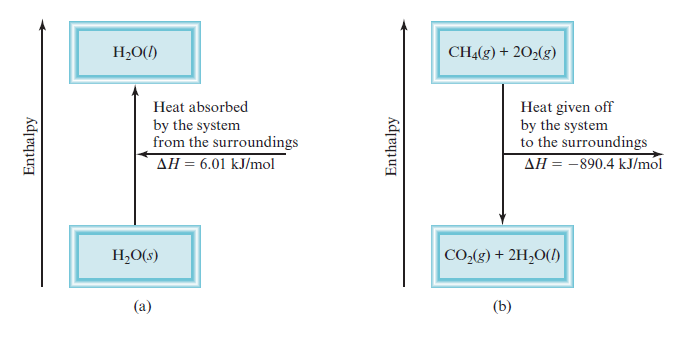
\includegraphics[width=0.5\textwidth]{Screenshot 2023-03-27 012722.png}
\end{figure}\\
(a) Melting 1 mole of ice at 0°C (an endothermic process) results in an enthalpy
increase in the system of 6.01 kJ. (b) Burning 1 mole of methane
in oxygen gas (an exothermic process) results in an enthalpy
decrease in the system of 890.4 kJ. Parts (a) and (b) are not drawn to
the same scale.\\ 
\begin{enumerate}
\item $\mathrm{CH}_{4}(g)+2 \mathrm{O}_{2}(g) \longrightarrow \mathrm{CO}_{2}(g)+2 \mathrm{H}_{2} \mathrm{O}(l)$;\\
$\Delta H=-890.4 \mathrm{~kJ} / \mathrm{mol}$
\item $\mathrm{CH}_{4}(g)+2 \mathrm{O}_{2}(g) \longrightarrow \mathrm{CO}_{2}(g)+2 \mathrm{H}_{2} \mathrm{O}(g)$;\\
$\Delta H=-802.4 \mathrm{~kJ} / \mathrm{mol}$
\item
$2 \mathrm{H}_{2} \mathrm{O}(l) \longrightarrow 2 \mathrm{H}_{2} \mathrm{O}(g)$;
$\Delta H=88.0 \mathrm{~kJ} / \mathrm{mol}$

\end{enumerate}


\section{Standard Enthalpy of \\ Reaction}
\begin{itemize}
\item The importance of the standard enthalpies of formation is that once we know their values, we can readily calculate the \textbf{standard enthalpy of reaction}. 
\item The \textbf{standard enthalpy of reaction}, $\mathrm{\Delta H_{\mathrm{rxn}}^{\circ}}$ is defined as the enthalpy of a reaction carried out at 1 atm.
\item For example, consider the hypothetical reaction.
$$\ce{aA + bB -> cC + dD}$$
where a, b, c, and d are stoichiometric coefficients. 
\item For this reaction $\mathrm{\Delta H_{\mathrm{rxn}}^{\circ}}$ is given by
\begin{center}
$\mathrm{\Delta H_{\mathrm{rxn}}^{\circ}=\left[c \Delta H_{\mathrm{f}}^{\circ}(\mathrm{C})+d \Delta H_{\mathrm{f}}^{\circ}(\mathrm{D})\right]}$ \\ 
$\mathrm{- \left[a \Delta H_{\mathrm{f}}^{\circ}(\mathrm{A})+b \Delta H_{\mathrm{f}}^{\circ}(\mathrm{B})\right]}$
\end{center}
\item We can generalize Equation as
\begin{center}
$\mathrm{\Delta H_{\mathrm{rxn}}^{\circ}=\Sigma n \Delta H_{\mathrm{f}}^{\circ}(\text { products })}$ \\
$\mathrm{-\Sigma m \Delta H_{\mathrm{f}}^{\circ}(\text { reactants })}$
\end{center}
where m and n denote the stoichiometric coefficients for the reactants and products.
\end{itemize}

\section{Determination of Standard Enthalpies of Formation and Reaction}
\begin{itemize}
\item Direct Method
\item Indirect Method- Hess’s Law
\end{itemize}

\section{The Direct Method}
\begin{itemize}
\item This method of measuring DH°f works for compounds that can be readily synthesized from their elements. 
\item Suppose we want to know the enthalpy of formation of carbon dioxide. We must measure the enthalpy of the reaction when carbon (graphite) and molecular oxygen in their standard states are converted to carbon dioxide in its standard state:
$$\ce{C(graphite) + O(g) -> CO2 (g)}$$
$$ \mathrm{\Delta H_{\mathrm{rxn}}^{\circ}=-393.5 \mathrm{~kJ} / \mathrm{mol}}$$
\item We know from experience that this combustion easily goes to completion. Thus, we can write
$$\begin{aligned}
\mathrm{\Delta H_{\mathrm{rxn}}^{\circ}} & \mathrm{=\Delta H_{\mathrm{f}}^{\circ}\left(\mathrm{CO}_{2}, g\right) -}\\ 
& \mathrm{\left[\Delta H_{\mathrm{f}}^{\circ}(\mathrm{C}, \text { graphite })+\Delta H_{\mathrm{f}}^{\circ}\left(\mathrm{O}_{2}, g\right)\right]} \\
& \mathrm{=-393.5 \mathrm{~kJ} / \mathrm{mol}}
\end{aligned}$$
\item Because both graphite and $\ce{O2}$ are stable allotropic forms of the elements, it follows that $\Delta H_{\mathrm{f}}^{\circ}(\mathrm{C}, \text { graphite })$ and $\Delta H_{\mathrm{f}}^{\circ}\left(\mathrm{O}_{2}, g\right)$ are zero. Therefore,
$$\begin{array}{c}
\mathrm{\Delta H_{\mathrm{rxn}}^{\circ}=\Delta H_{\mathrm{f}}^{\circ}\left(\mathrm{CO}_{2}, g\right)=-393.5 \mathrm{~kJ} / \mathrm{mol}} \\
\mathrm{\Delta H_{\mathrm{f}}^{\circ}\left(\mathrm{CO}_{2}, g\right)=-393.5 \mathrm{~kJ} / \mathrm{mol}}
\end{array}$$
\end{itemize}

\section{The Indirect Method}
\begin{itemize}
\item Many compounds cannot be directly synthesized from their elements. 
\item In some cases, the reaction proceeds too slowly, or side reactions produce substances other than the desired compound. 
\item In these cases, $\mathrm{\Delta H_{\mathrm{f}}^{\circ}}$  can be determined by an \textbf{ indirect approach}.
\end{itemize}

\section{Hess’s Law of Heat Summation}
\begin{itemize}
\item When reactants are converted to products, the change in enthalpy is the same whether the reaction takes place in one step or in a series of steps.
\item If we can break down the reaction of interest into a series of reactions for which $\mathrm{\Delta H_{\mathrm{rxn}}^{\circ}}$ can be measured, we can calculate  $\mathrm{\Delta H_{\mathrm{rxn}}^{\circ}}$ for the overall reaction. 
\item Hess’s law is based on the fact that because H is a state function, DH depends only on the initial and final state (that is, only on the nature of reactants and products). The enthalpy change would be the same whether the overall reaction takes place in one step or many steps.
\end{itemize}

\section{Application of Hess’s Law}
\begin{figure}[h]
\centering
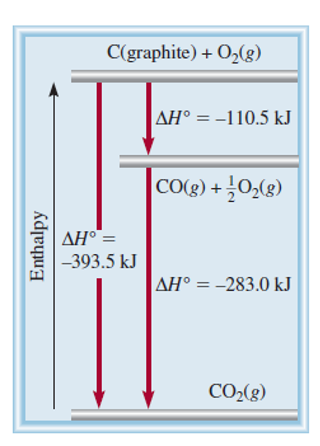
\includegraphics[width=1.5in,height=1.8in]{hess.png}
\end{figure}
The enthalpy change for the formation of 1 mole of $\ce{CO2}$ from graphite and $\ce{O2}$ can be broken down into two steps according to Hess’s law.
\begin{figure}[h]
\centering
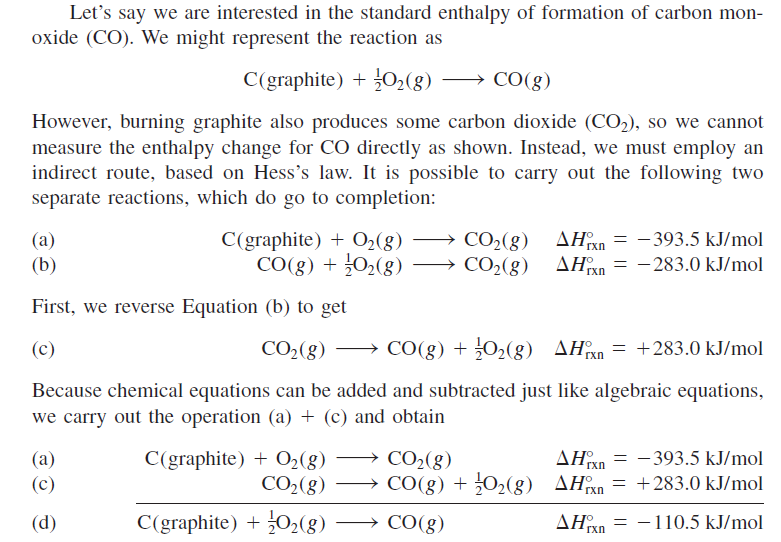
\includegraphics[width=0.5\textwidth]{Screenshot 2023-03-27 005925.png}
\end{figure}
Thus, $\Delta H_{\mathrm{f}}^{\circ}(\mathrm{CO})=-110.5 \mathrm{~kJ} / \mathrm{mol}$
\newline
{\large Why do chemical processes tend to favor one direction?}
\begin{Box1}{}
The second law of thermodynamics
\end{Box1}

\section{Spontaneous Processes}
\begin{itemize}
\item One of the main objectives in studying thermodynamics, as far as chemists are concerned, is to be able \textbf{to predict whether or not a reaction will occur} when reactants are brought together under a specific set of conditions (for example, at a certain temperature, pressure, and concentration).
\item A reaction that does occur under the given set of conditions is called a \textbf{spontaneous reaction}. 
\item If a reaction does not occur under specified conditions, it is said to be \textbf{nonspontaneous}.
\end{itemize}

\section{Examples of Spontaneous Physical and Chemical Processes}
\begin{itemize}
\item A waterfall runs downhill, but never up, spontaneously.
\item A lump of sugar spontaneously dissolves in a cup of coffee, but dissolved sugar does not spontaneously reappear in its original form.
\item Water freezes spontaneously below 0°C, and ice melts spontaneously above 0°C (at 1 atm).
\item Heat flows from a hotter object to a colder one, but the reverse never happens spontaneously.
\item The expansion of a gas into an evacuated bulb is a spontaneous process. The reverse process, that is, the gathering of all the molecules into one bulb, is not spontaneous.
\item A piece of sodium metal reacts violently with water to form sodium hydroxide and hydrogen gas. However, hydrogen gas does not react with sodium hydroxide to form water and sodium.
\item Iron exposed to water and oxygen forms rust, but rust does not spontaneously change back to iron.
\end{itemize}

\begin{figure}[h]
\centering
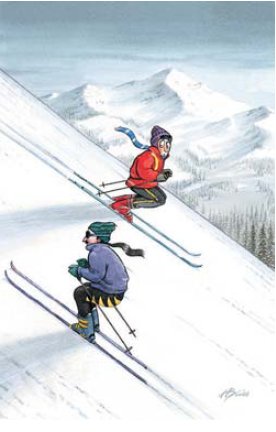
\includegraphics[width=1.5in, height=2in]{ski.png}
\end{figure}
A spontaneous and a nonspontaneous process.
\begin{figure}[h]
\centering
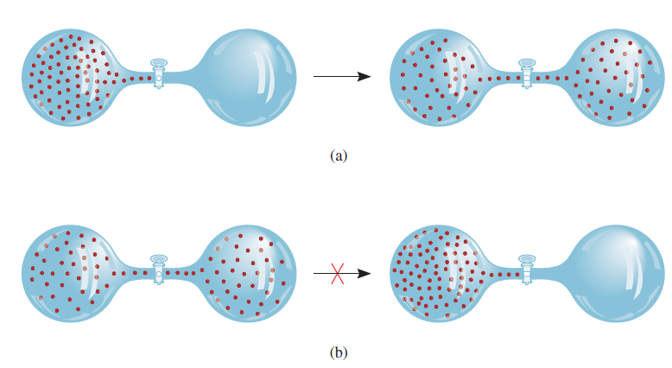
\includegraphics[width=0.5\textwidth]{spontanity.png}
\end{figure}
(a) A spontaneous process. After the valve is opened, the molecules distribute evenly between the two bulbs. (b) A nonspontaneous process. After the valve is opened, the molecules preferentially gather in one bulb.
\\
\\
\begin{Box1}{}
{\large Processes that occur spontaneously in one direction \textbf{cannot}, under the same conditions, also take place spontaneously in the opposite direction.}
\end{Box1}

\section{Exothermicity and Spontaneity}
\begin{itemize}
\item If we assume that spontaneous processes occur so as to decrease the energy of a system.
\item A large number of exothermic reactions are spontaneous. An example is the combustion of methane:
$$\ce{CH4 (g) + 2O2 (g) -> CO2 (g) + 2H2O (l)}$$
$$\mathrm{\Delta H^{\circ} = -890.4 \text{ kJ/mol}}$$
\item Another example is the acid-base neutralization reaction:
$$\ce{H^+ (aq) + OH^- (aq) -> H2O (l)}$$
$$\mathrm{\Delta H^{\circ} = -56.2 \text{ kJ/mol}}$$
\end{itemize}
\section{Endothermicity and Spontaneity}
\begin{itemize}
    \item Consider a solid-to-liquid phase transition such as
$$\ce{H2O (s) -> H2O (l)}$$
$$\mathrm{\Delta H^{\circ} = 6.01 \text{ kJ/mol}}$$
    In this case, \textbf{the assumption that spontaneous processes always decrease energy of a system fails}. Experience tells us that ice melts spontaneously above 0°C even though the process is endothermic.
\item Another example that contradicts our assumption is the dissolution of ammonium nitrate in water:
$$\ce{NH4NO3 (s) ->[H2O] NH^{+}4 (aq) + NO^{-}3 (aq)}$$
$$\mathrm{\Delta H^{\circ} = 25 \text{ kJ/mol}}$$
This process is spontaneous, and yet it is also endothermic.
\item   The decomposition of mercury(II) oxide is an endothermic reaction that is nonspontaneous at room temperature, but it becomes spontaneous when the temperature is raised:
$$\ce{2HgO(s) -> 2Hg(l) + O2(g)}$$
$$\mathrm{\Delta H^{\circ} = 90.7 \text{ kJ/mol}}$$
\end{itemize}

\section{Spontaneity and Entropy}
\begin{itemize}
\item Exothermicity favors the spontaneity of a reaction but does not guarantee it. 
\item Just as it is possible for an endothermic reaction to be spontaneous, it is possible for an exothermic reaction to be nonspontaneous. \textbf{Combustion reactions} are good examples of exothermic reactions that are also nonspontaneous. For example, the combustion of methane with oxygen gas to produce carbon dioxide and water (CH4(g) + 2O2(g) --> CO2(g) + 2H2O(g)) is exothermic because it releases heat, but it is nonspontaneous because it requires an external heat source to proceed with the forward reaction.
\item We \textbf{cannot decide whether or not a chemical reaction will occur spontaneously solely on the basis of energy changes in the system.} 
\item To make this kind of prediction we need another thermodynamic quantity, which turns out to be \textbf{entropy}.
\end{itemize}

\section{Entropy}
\begin{itemize}
\item Entropy (S) is described as a measure of how spread out or dispersed the energy of a system is among the different possible ways that system can contain energy. 
\item The greater the dispersal, the greater is the entropy.
\item Most processes are accompanied by a change in entropy.
\end{itemize}
\section{Entropy-Example}
\begin{itemize}

\item A cup of hot water has a certain amount of entropy due to the dispersal of energy among the various energy states of the water molecules (for example, energy states associated with the translational, rotational, and vibrational motions of the water molecules). 
\item If left standing on a table, the water loses heat to the cooler surroundings. 
\item Consequently, there is an overall increase in entropy because of the dispersal of energy over a great many energy states of the air molecules.
\begin{figure}[h]
\centering
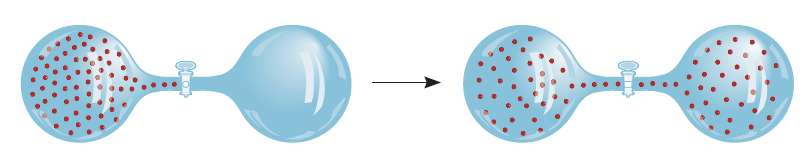
\includegraphics[width=0.5\textwidth]{Screenshot 2023-03-27 004722.png}
\end{figure}
\item Before the valve is opened, the system possesses a certain amount of entropy. 
\item Upon opening the valve, the gas molecules now have access to the combined volume of both bulbs. 
\item A larger volume for movement results in a narrowing of the gap between translational energy levels of the molecules. 
\item Consequently, the entropy of the system increases because closely spaced energy levels leads to a greater dispersal among the energy levels.
\end{itemize}

\section{Standard Entropy}
\begin{itemize}
\item Entropy is obtained by calorimetric methods. 
\item It is possible to determine the absolute value of entropy of a substance, called \textbf{absolute entropy}. 
\item \textbf{Standard entropy} is the absolute entropy of a substance at 1 atm and 25°C.
\end{itemize}

\section{The Second Law of Thermodynamics}
    The connection between entropy and the spontaneity of a reaction is expressed by the second law of thermodynamics:
    \begin{Box1}{}
    \textbf{
       The entropy of the universe increases in a spontaneous process and remains unchanged in an equilibrium process.}
     \end{Box1} 
   
\section{Mathematical Expression of The Second Law of Thermodynamics}
\begin{itemize}
\item Because the universe is made up of the system and the surroundings, the entropy change in the universe ($\mathrm{\Delta S_{univ}}$) for any process is the sum of the entropy changes in the system ($\mathrm{\Delta S_{sys}}$) and in the surroundings ($\mathrm{\Delta S_{surr}}$). We can express the second law of thermodynamics as follows:
\begin{table}[h]
\centering
\def\arraystretch{1.5}
\begin{tabular}{|p{1.2in}|l|}
\hline
For a spontaneous process: & $\mathrm{\Delta S_{univ} = \Delta S_{sys} + \Delta S_{surr} > 0}$ \\ \hline
For an equilibrium process: & $\mathrm{\Delta S_{univ} = \Delta S_{sys} + \Delta S_{surr} = 0}$ \\ \hline
\end{tabular}
\end{table}
\item For a spontaneous process, the second law says that $\mathrm{\Delta S_{univ}}$ must be greater than zero, but it does not place a restriction on either $\mathrm{\Delta S_{sys}}$ or $\mathrm{\Delta S_{surr}}$. Thus, it is possible for either $\mathrm{\Delta S_{sys}}$ or $\mathrm{\Delta S_{surr}}$ to be negative, as long as the sum of these two quantities is greater than zero. For an equilibrium process, $\mathrm{\Delta S_{univ}}$ is zero. In this case, $\mathrm{\Delta S_{sys}}$ and $\mathrm{\Delta S_{surr}}$ must be equal in magnitude, but opposite in sign. 
\item What if for some hypothetical process we find that $\mathrm{\Delta S_{univ}}$ is negative? What this means is that the process is not spontaneous in the direction described. Rather, it is spontaneous in the opposite direction.
\end{itemize}

\section{Entropy Changes in The System}
\begin{itemize}
\item To calculate $\mathrm{\Delta S_{univ}}$, we need to know both $\mathrm{\Delta S_{sys}}$ and $\mathrm{\Delta S_{surr}}$. Let us focus first on  $\mathrm{\Delta S_{sys}}$. Suppose that the system is represented by the following reaction:
$$\ce{aA + bB -> cC + dD}$$
\item The standard entropy of reaction  $\mathrm{\Delta S_{rxn}^{\circ}}$ is given by the difference in standard entropies between products and reactants:
$$\Delta S_{\mathrm{rxn}}^{\circ}=\left[c S^{\circ}(\mathrm{C})+d S^{\circ}(\mathrm{D})\right]-\left[a S^{\circ}(\mathrm{A})+b S^{\circ}(\mathrm{B})\right]$$
or, in general, using $\sum$ to represent summation and m and n for the stoichiometric coefficients in the reaction
$$\Delta S_{\mathrm{rxn}}^{\circ}=\Sigma n S^{\circ}(\text { products })-\Sigma m S^{\circ}(\text { reactants })$$
\end{itemize}

\section{Entropy Changes in the Surroundings}
\begin{figure}[h]
\centering
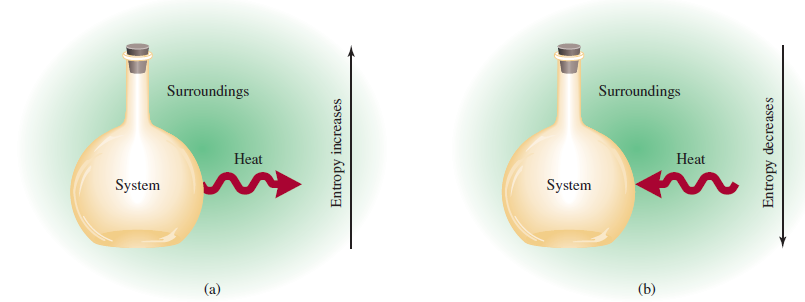
\includegraphics[width=0.5\textwidth]{Screenshot 2023-03-27 004429.png}
\end{figure}
(a) An exothermic process transfers heat from the system to the surroundings and results in an increase in the entropy of the surroundings. (b) An endothermic process absorbs heat from the surroundings and thereby decreases the entropy of the surroundings.
\section{New Thermodynamic Function}
\begin{itemize}
\item The second law of thermodynamics tells us that a spontaneous reaction increases the entropy of the universe; that is, $\mathrm{\Delta S_{univ} > 0}$. In order to determine the sign of $\mathrm{\Delta S_{univ}}$ for a reaction, however, we would need to calculate both $\mathrm{\Delta S_{sys}}$ and $\mathrm{\Delta S_{surr}}$. 
\item In general, we are usually concerned only with what happens in a particular system. 
\item Therefore, we need another thermodynamic function to help us determine whether a reaction will occur spontaneously if we consider only the system itself.
\end{itemize}

\section{Gibbs Free Energy}
\begin{itemize}
\item For a spontaneous process,
\begin{Box1}{}
$\begin{array}{c}
\Delta S_{\text {univ }}=\Delta S_{\mathrm{sys}}+\Delta S_{\mathrm{surr}}>0 \\
\Delta S_{\text {univ }}=\Delta S_{\mathrm{sys}}- \dfrac{\Delta H_{\mathrm{sys}}}{T}>0 \\
T \Delta S_{\text {univ }}=-\Delta H_{\mathrm{sys}}+T \Delta S_{\mathrm{sys}}>0 \\
-T \Delta S_{\text {univ }}=\Delta H_{\mathrm{sys}}-T \Delta S_{\mathrm{sys}}<0
\end{array}$
\end{Box1}
\item For a process carried out at constant pressure and temperature T, if the changes in enthalpy and entropy of the system are such that $\mathrm{\Delta H_{\mathrm{sys}}-T \Delta S_{\mathrm{sys}}}$ is less than zero, the process must be spontaneous.
\item In order to express the spontaneity of a reaction more directly, we introduce another thermodynamic function called \textbf{Gibbs free energy (G)}, or simply \textbf{free energy:}
$$\mathrm{G = H - TS}$$
\end{itemize}

\section{Change in Free Energy of a System for a Constant-Temperature Process}
$$\mathrm{\Delta G = \Delta H - T \Delta S}$$
\begin{itemize}
\item Free energy is the energy available to do work. 
\item If a particular reaction is accompanied by a release of usable energy (that is, if $\mathrm{\Delta G}$ is negative), this fact alone guarantees that it is spontaneous, and there is no need to worry about what happens to the rest of the universe. 
\item It is impossible to measure all these contributions accurately, so we cannot calculate the total energy of a system with any certainty.  Changes in energy, on the other hand, can be determined experimentally.
\end{itemize}

\section{Conditions for Spontaneity and Equilibrium}
Conditions for spontaneity and equilibrium at constant temperature and pressure in terms of $\mathrm{\Delta G}$ are:
\begin{enumerate}
\item $\mathbf{\Delta G < 0}$: The reaction is spontaneous in the forward direction.
\item $\mathbf{\Delta G > 0}$: The reaction is nonspontaneous. The reaction is spontaneous in the opposite direction.
\item $\mathbf{\Delta G = 0}$: The system is at equilibrium. There is no net change.
\end{enumerate}
\section{Standard Free Energy Changes}
\begin{itemize}
\item The standard free-energy of reaction ($\mathrm{\Delta G_{\mathrm{rxn}}^{\circ}}$) is the free-energy change for a reaction when it occurs under standard-state conditions, when reactants in their standard states are converted to products in their standard states.
$$a \mathrm{~A}+b \mathrm{~B} \longrightarrow c \mathrm{C}+d \mathrm{D}$$
\begin{center}
$\mathrm{\Delta G_{\mathrm{rxn}}^{\circ}=\left[c \Delta G_{\mathrm{f}}^{\circ}(\mathrm{C})+d \Delta G_{\mathrm{f}}^{\circ}(\mathrm{D})\right]}$\\
$\mathrm{-\left[a \Delta G_{\mathrm{f}}^{\circ}(\mathrm{A})+b \Delta G_{\mathrm{f}}^{\circ}(\mathrm{B})\right]}$
\end{center}
\item We can generalize the equation as:
\begin{center}{c}
$\mathrm{\Delta G_{\mathrm{rxn}}^{\circ}=\Sigma n \Delta G_{\mathrm{f}}^{\circ}(\text { products })}$\\
$\mathrm{-\Sigma m \Delta G_{\mathrm{f}}^{\circ}(\text { reactants })}$
\end{center}
where m and n are stoichiometric coefficients. 
\item The term $\mathrm{\Delta G_{\mathrm{f}}^{\circ}}$  is \textbf{the standard free energy of formation of a compound}, that is, \textbf{the free-energy change that occurs when 1 mole of the compound is synthesized from its elements in their standard states.}
\end{itemize}

{\large Factors Affecting the Sign of $\Delta G$ in the Relationship $\Delta G = \Delta H - T\Delta S$}
\begin{table}[h]
\centering
\def\arraystretch{1.5}
\begin{tabular} {|l|l|p{2.3in}|}
\hline
$\Delta H$ & $\Delta S$ & $\Delta G$ \\ \hline
+ & + & Reaction proceeds spontaneously at high temperatures. At low temperatures, reaction is spontaneous in the reverse direction. example: $$\ce{2HgO (s) -> 2Hg (l) + O2 (g)}$$ \\ \hline
+ & - & $\Delta G$ is always positive. Reaction is spontaneous in the reverse direction at all temperatures. example: $$\ce{3O2 (g) -> 2O3 (g)}$$ \\ \hline

\end{tabular}
\end{table}

\begin{table}[h]
\centering
\def\arraystretch{1.5}
\begin{tabular} {|l|l|p{2.3in}|}
\hline
$\Delta H$ & $\Delta S$ & $\Delta G$ \\ \hline
- & + & $\Delta G$ is always negative. Reaction proceeds spontaneously at all temperatures. example: $$\ce{2H2O2 (aq) -> 2H2O(l) + O2(g)}$$ \\ \hline
- & - & Reaction proceeds spontaneously at low temperatures. At high temperatures, the reverse reaction becomes spontaneous.  $$\ce{NH3 (g) + HCl (g) -> NH4Cl(s)}$$\\ \hline
\end{tabular}
\end{table}

\section{Carnot Cycle}
\begin{itemize}
\item The Carnot cycle is a theoretical ideal \textbf{thermodynamic cycle} proposed by French physicist \textbf{Sadi Carnot} in 1824 and expanded upon by others in the 1830s and 1840s. 
\item It provides an upper limit on the efficiency that any classical thermodynamic engine can achieve during the conversion of heat into work, or conversely, the efficiency of a refrigeration system in creating a temperature difference by the application of work to the system. 
\end{itemize}
{\large Mechanism Of Carnot Cycle:}
\begin{figure}[h]
\centering
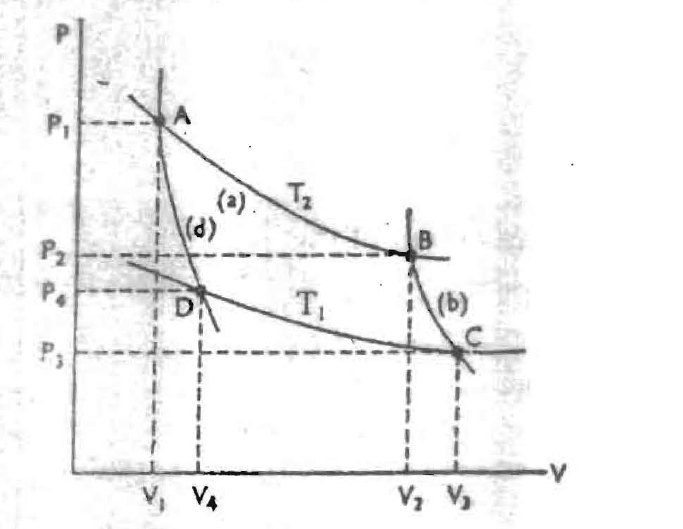
\includegraphics[width=0.5\textwidth]{Screenshot 2023-03-27 003237.png}
\end{figure}
\begin{center}
The Carnot Cycle on a P-V diagram.
\end{center}
\begin{Box1}{}
\small
Step 1: Isothermal expansion at temperature $T_2$\\
Step 2: Adiabatic expansion to temperature $T_l$\\
Step 3: Isothermal compression at temperature $T_1$ and\\
Step 4: Adiabatic compression backto the original temperature $T_2$
\end{Box1}
\textbf{Step 1:} The cylinder is placed in the heat reservoir at temperature $T_2$ and the gas allowed to expand isothermally and reversibly until its pressure and volume change from $P_l$ and $V_l$ to $P_2$ and $V_2$ respectively. The gas absorbs heat from the reservoir and performs work $w_1$. For this step:
Heat absorbed $=q_2$, and since the gas is ideal and expands isothermally, $\Delta U=0$.
$$
\text { work }=w_1=-R T_2 \ln  \dfrac{V_2}{V_1}
$$
\textbf{Step 2:} The cylinder containing the gas at a pressure $P_2$, volume $V_2$ and temperature $T_2$ is now placed in the insulated vessel and further expanded adiabatically to a volume $V_3$ when the pressure falls to $P_3$. The temperature of the gas falls to $T_1$, as the temperature falls during an adiabatic expansion. Let the work done by the gas as a result of this expansion be $w_2$. Since the cylinder is placed in an insulated vessel no heat is absorbed, i.e. $q=0$. In this step
$$
\text {Work done}=w_2=\Delta U=\int_{T_2}^{T_1} C_V d T=C_V\left(T_1-T_2\right)
$$
or,
$$
w_2=C_V\left(T_1-T_2\right) .
$$
\textbf{Step 3:} The cylinder is now placed in the heat reservoir at $T_I$ and the gas is compressed adiabatically and reversibly from volume $V_3$ to wolume $V_4$, the pressure changing from $P_3$ to $P_4$. An amount of work $w_3$ is done on the gas by the piston, and an amount of heat $q_1$ is given out by the gas to the reservoir at temperature $T_1$. In this step
Heat change $=q_1\left(q_1\right.$ is a negative quantity, since heat is given out)
$$
w_3=-R T_1 \ln  \dfrac{V_4}{V_3}
$$
$$\Delta U=0, \quad$$ since the process is isothermal.
\newline
\newline
\textbf{Step 4:} The cylinder of gas, now at temperature $T_l$, is again placed in the insulated vessel. The gas is compressed adiabatically and reversibly from volume $V_4$ to the original volume $V_l$; the temperature rises to $T_2$ and the pressure changes from $P_4$ to $P_7$. An amount of work, $w_4$, is done on the gas and no heat is given out or absorbed, i.e. $q=0$. Now the gas is in the same state as at the start of Step I. For this step:\\
Heat change $q=0$,
$$
w_4=\Delta U=\int_{T_1}^{T_2} C_V d T=C_V\left(T_2-T_1\right)
$$
The cycle is now complete as the gas has returned to its original state. The total work one by the gas during the cycle is
$$
W_{\text {Total }}=w_1+w_2+w_3+w_4
$$
Also $w_2$ and $w_4$, being numerically equal but opposite in sign, cancel each other. The net work done by the system is, therefore,
$$
\begin{aligned}
& W_{n e t}=w_1+w_3 \\
&=-R T_2 \ln  \dfrac{V_2}{V_1}+\left(-R T_1 \ln  \dfrac{V_4}{V_3}\right) \\
&=-R T_2 \ln  \dfrac{V_2}{V_1}-R T_1 \ln  \dfrac{V_4}{V_3} \\
& \text { Or, }-W_{n e t}=R T_2 \ln  \dfrac{V_2}{V_1}+R T_1 \ln  \dfrac{V_4}{V_3} \\
\end{aligned}
$$

It can be seen from figure that $V_{1}$ and $V_4$ lie on one adiabatic curve, while $V_2$ and $V_3$ lie on another curve. It can be shown by applying temperature-volume relationship for adiabatic processes that,
$$
\left(\frac{V_3}{V_2}\right)^{\gamma-1}=\frac{T_2}{T_1} \text { and }\left(\frac{V_4}{V_1}\right)^{\gamma-1}=\frac{T_2}{T_1}
$$
Combining these two equations we get,
$$
\frac{V_3}{V_2}=\frac{V_4}{V_1}, \quad \text { or } \quad \frac{V_4}{V_3}=\frac{V_1}{V_2}
$$
On substitution of equations and rearranging we get,
$$
\begin{aligned}
&-W_{\text {net }}=R T_2 \ln \frac{V_2}{V_1}+R T_1 \ln \frac{V_4}{V_3} \\
\Rightarrow &-W_{\text {net }}=R T_2 \ln \frac{V_2}{V_1}+R T_1 \ln \frac{V_l}{V_2} \\
\Rightarrow &-W_{\text {net }}=R T_2 \ln \frac{V_2}{V_1}-R T_1 \ln \frac{V_2}{V_l} \\
\Rightarrow &-W_{\text {net }}=R\left(T_2-T_l\right) \ln \frac{V_2}{V_l}
\end{aligned}
$$
Since this is a positive quantity, $W_{net}$ gives the net amount of work produced per cycle. In other words heat is being converted into work.
Again, in Step 1, the work done is equal to heat absorbed $q_2$, i.e.,
$$
q_2=R T_2 \ln \frac{V_2}{V_l}
$$
From above equations, one obtains,
$$
\frac{W_{n e t}}{q_2}=\frac{R\left(T_2-T_1\right) \ln \left(V_2 / V_1\right)}{R T_2 \ln \left(V_2 / V_l\right)}=\frac{T_2-T_1}{T_2}
$$


\section{Heat Engine}
\begin{itemize}
\item Heat engine is a device that exploits a temperature difference to perform work. 
\item When two systems at different temperatures are placed in contact with one another, heat energy transfer will take place between them. 
\end{itemize}

\section{Efficiency of Heat Engine}
$$\text{Efficiency} = \dfrac{\text{Work done}}{\text{Heat Energy Transferred in}}$$
\begin{Box1}{}
$\text{Efficiency} = \mathrm{\eta} = \dfrac{\mathrm{Q_{Hot} - Q_{Cold}}}{\mathrm{Q_{Hot}}} = 1 -\dfrac{\mathrm{Q_{Cold}}}{\mathrm{Q_{Hot}}}$
\end{Box1}

\section{How does a heat engine work?}
\begin{figure}[h]
\centering
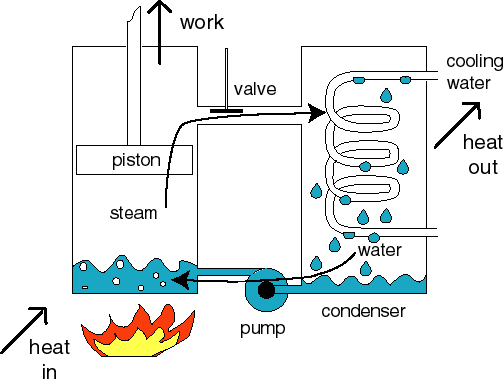
\includegraphics[width=0.5\textwidth]{heatengine.png}
\end{figure}

\section{Third Law of Thermodynamics} 
\begin{Box1}{}
\textbf{The entropy of a perfect crystalline substance is zero at the absolute zero of temperature.}
\end{Box1}

\begin{itemize}
\item Entropy is related to microstates—the greater the number of microstates a system possesses, the larger is the entropy of the system. 
\item Consider a perfect crystalline substance at absolute zero (0 K). Under these conditions, molecular motions are kept at a minimum and the number of microstates (W) is one (there is only one way to arrange the atoms or molecules to form a perfect crystal).
\end{itemize}
$$\begin{aligned}
S & =k \ln W \\
& =k \ln 1=0
\end{aligned}$$




\section{Absolute Entropy}
\begin{itemize}
\item The third law of thermodynamics enables us to determine the absolute entropies of substances.
 \item Starting with the knowledge that the entropy of a pure crystalline substance is zero at absolute zero, we can measure the increase in entropy of the substance when it is heated from 0 K to, say, 298 K. The change in entropy, $\mathrm{\Delta S}$, is given by:
 $$\begin{aligned}
\Delta S & =S_{\mathrm{f}}-S_{\mathrm{i}} \\
& =S_{\mathrm{f}}
\end{aligned}$$
\end{itemize}

\textbf{Entropy increase of a substance as the temperature rises from absolute zero.}
\begin{figure}[h]
\centering
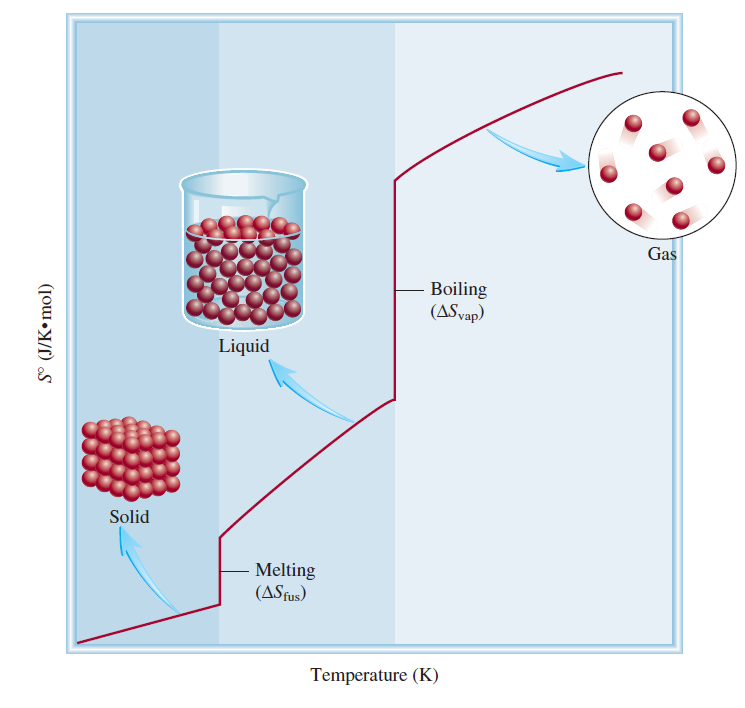
\includegraphics[width=0.5\textwidth]{Screenshot 2023-03-27 004224.png}
\end{figure}

\end{document}


